\section{Anexo Manifestaciones seguras}

En una decisión temeraria una ciudad decidió autorizar un conjunto de n manifestaciones el mismo día y horas. Cada manifestación comienza en un punto de reunión y tiene un destino final. Para evitar enfrentamientos y confusiones desean que cada ruta sea aislada de las otras. Contamos con el mapa de la ciudad que incluye todos los caminos e intersecciones por los que pueden ir las marchas. Nos piden que elaboremos un algoritmo que retorne los caminos a seguir para cada manifestación de modo que no haya riesgo de un cruce (si es posible).\newline
Debemos demostrar que es un problema NP-Completo.
%=============================================

\subsection{Solución}
El problema que precede se puede modelar con un grafo en donde los nodos son las intersecciones de las calles y las aristas son las calles de la ciudad. En un principio todas las calles están disponibles para efectuar las manifestaciones siempre y cuando no se superpongan las manifestaciones.
%=============================================

\subsection{Demostración NP-Completo}
Para demostrar que es $\mathsf{NP-Completo}$ debemos demostrar que nuestro problema pertenece a $\mathsf{NP}$ y a $\mathsf{NP-Hard}$ simultáneamente.

\subsubsection{Demostración NP}
Para demostrar que el problema es $\mathsf{NP}$ debemos poder corroborar la solución propuesta en tiempo polinomial. Usando la analogía de la cerradura y la llave, esto sería equivalente a dada la llave probar que esta abre la cerradura en "tiempo polinomial". \newline

A continuación se propone un algoritmo que verifica la solución propuesta en tiempo polinomial:

\begin{verbatim}
Llamar L a la lista de manifestaciones(representadas por tuplas ordenadas de nodos)

Funcion esManifestacionValida(L):
    Llamo C al grafo que representa a la ciudad
    Llamar visitados a la lista que contendrá a los nodos visitados
    
    visitados es lista vacia
    Para cada manifestacion en L:
        Para cada esquina en manifestacion:
            Llamo S a siguiente esquina
            Si esquina en visitados:
                Devolver falso
            Si existe S y no existe camino(esquina,S):
                Devolver falso
            Sino:
                visitados agregar esquina
    Devolver verdadero
\end{verbatim}

Se puede apreciar que la complejidad es de $\mathcal{O}(km)$ siendo $k$ la cantidad de manifestaciones y $m$ la cantidad máxima de esquinas atravesadas por una manifestación.

\subsubsection{Demostración NP-Hard}
Para demostrar que el problema es $\mathsf{NP-Hard}$, consideremos una instancia del problema 3-SAT compuesto por $m$ clausuras y $n$ variables:\newline

$E = (X_{1}+X_{2}+X_{3})*(\overline{X_{1}}+\overline{X_{2}}+\overline{X_{4}})*(\overline{X_{2}}+\overline{X_{3}}+X_{4})$\newline

Para crear el grafo en el que se resolverá el problema de las manifestaciones definimos para cada variable ($i$ de $1$ a $n$) y para cada clausura ($j$ de $1$ a $m$) dos vértices: $X_{ij}$ ($true$) y $\overline{X_{ij}}$ ($false$); creando así 6 vértices por clausura. A su vez definimos un par de vértices $I$ (inicio) y $F$ (fin) por cada clausura y por cada variable quedándonos así formados los pares $I_{jc}$, $F_{jc}$ (para los pares de las clausuras) y $I_{iv}$, $F_{iv}$ (para los pares de las variables).\newline

Por cada clausura conectaremos $I_{jc}$ a $X_{ij}$ si la variable $X_{ij}$ esta sin negar y por consiguiente a $\overline{X_{ij}}$ si la variable esta negada y luego conectaremos la variable $X_{ij}$ usada al $F_{jc}$ correspondiente.\newline

Por cada variable conectaremos $I_{iv}$ al vértice $X_{ij}$ cuya $j$ sea la clausura de menor índice en la que aparezca la variable $i$, después conectaremos dicho $X_{ij}$ al $X_{ij}$ cuya $j$ sea la segunda clausura de menor índice en el que aparezca la variable $i$, crearemos aristas hasta que ya no queden clausuras que utilicen la variable $i$ y procederemos a unir el ultimo $X_{ij}$ al $F_{iv}$. Realizaremos exactamente el mismo procedimiento con las variables $\overline{X_{ij}}$. \newline

De esta forma nos queda el siguiente grafo: \newline

\begin{figure}[H]
\centering
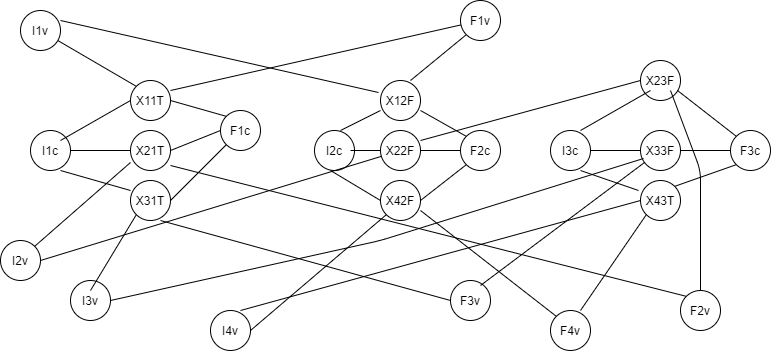
\includegraphics[width=0.9\textwidth]{Informe/Imagenes/Parte1/grafico 2-bis.png}
\caption{\label{fig:class01} Grafo manifestaciones}
\end{figure}

\underline{Nota:} No se muestran en el grafo los $X_{ij}$ que se encuentran aislados del resto para no sobrecargar al mismo y facilitar su comprensión.\newline

Por ultimo definiremos las manifestaciones. Existirá una manifestación por clausura, esta iniciara en el nodo $I_{jc}$ y finalizara en el $F_{jc}$ y otra manifestación por cada variable la cual iniciara en el nodo $I_{iv}$ y finalizara en el $F_{iv}$.\newline

Entonces en relación al problema de 3-SAT el camino que tomen las manifestaciones de las clausuras será la evaluación literal de $true$ de la variable y el camino que no usemos de las manifestaciones de las variables corresponderá a la asignación de $true$ a la variable. \newline

%=============================================


